\section{Methods}
In the following, the foundational concepts used within this thesis are outlined in detail. The proposed model, FlowCoder, is introduced and an exact computational model is given, before describing implementational details and training and testing strategies.
\subsection{Foundations \& Computational Framework}

\paragraph*{\acrshort{gfn}} \acrshortpl{gfn} create a \acrfull{dag} over the state space, where vertices correspond to states or partial samples and edges denote transitions or adding a component to a partial sample, in which the edges carry a flow from source to targets \cite{bengioFlowNetworkBased2021}.
In \acrshortpl{gfn}, the "flow" in the network corresponds to the process by which the network constructs a sample, which can be thought of as a path in a graph where nodes are partial samples, and edges correspond to adding a component to the partial sample.
The core training objective for a \acrshort{gfn} is to satisfy the flow matching constraint. The idea is to ensure that the flow into any state (a partially constructed sample) matches the flow out of it, given the reward associated with complete samples. The flow here refers to the expected transitions into or out of a state under the model's stochastic policy. 

Formally, a state \( s \) represents a partial object a certain stage in the generative process. A trajectory \( \tau \) is a sequence of states \( s_0, s_1, ..., s_T \); the model traverses from an initial state \( s_0 \) to a terminal state \( s_T \), where the target structure is complete.
A trajectory \( \tau \) is formed by a sequence of actions \( a_1, a_2, ..., a_T \), where each action \( a_t \) transitions the model from state \( s_{t} \) to state \( s_{t+1} \). The sequence of actions is governed by a policy \( \pi \), which defines the probability of choosing a particular action given the current state.
The flow \( F(\tau) \) of a trajectory \( \tau \) is defined as the product of the probabilities of each transition along the trajectory, multiplied by the reward \( R(s_T) \) of the terminal state, normalized by a partition function \( Z \).

\begin{equation} \label{eq:flow}
    F(\tau) = \frac{R(s_T)}{Z} \prod_{t=0}^{T-1} \pi_\phi(s_{t+1} | s_{t})
\end{equation}

The partition function \( Z \) ensures that the sum of flows over all possible trajectories equals one, effectively normalizing the distribution. Since we don't know \( Z \), we can estimate it by parameterizing it as \( Z_{\theta} \).
The flow matching constraint enforces that for any given non-terminal state \( s \), the total flow into \( s \) must equal the total flow out of \( s \):

\begin{equation} \label{eq:flow_match}
    F(\tau) = F(\tau')
\end{equation}

where \( F(\tau') \) is the reverse trajectory. The partition function is estimated and utilized to balance the probabilities throughout the \acrshort{dag}.
Following \citet{malkinTrajectoryBalanceImproved2022}, we can utilize this property to create a suitable loss function - \acrfull{tb} Loss to train the \acrshort{gfn}. 

\begin{equation}\label{form:TB}
    \mathcal{L}_{TB} = \left(\log Z_\theta(x) + \sum_{t=0}^{T-1} \log \pi_\phi(s_{t+1}|s_{t}, x) - \log R(s_T \vert x)\right)^2
\end{equation}     

Here $s_T$ is a constructed object, in this case a program $\rho$. The complete derivation of the TB loss can be found in \autoref{app:TB}. \\
To compute the reward $R(\rho | x)$, the sampled program $\rho$ is executed and evaluated to get $\rho(x_{in}) = \tilde{x}_{\text{out}}$ after which the output pair $(x_{\text{out}}, \tilde{x}_{\text{out}})$ is compared. \\
Additionally, a state-task representation is encoded by $T_\theta(x, s_t)$, parameterized by $\theta$. In this project, $T$ will be referred to as state-task representation or generative model interchangeably. The output $z = T_\theta(x, s_t)$ is the task-state representation which policy $\pi$ takes as an input.

\paragraph*{\acrfull{em}} \acrlong{em} is an algorithm for finding maximum likelihood estimates in models with latent variables. It iteratively optimizes a lower bound on the likelihood of the observed data, alternating between inferring the most likely latent states (E-step) and optimizing model parameters given these states (M-step) \cite{han2022data}. \acrshort{em} has been used repeatedly in in the realms of grammar induction or program synthesis. DreamCoder uses a generalized version of \acrshort{em} \cite{ellisDreamCoderBootstrappingInductive2021}. \citet{kimCompoundProbabilisticContextFree2019} use \acrshort{em} for grammar induction and \citet{Hu_Malkin_Jain_Everett_Graikos_Bengio_2023} extend \citeauthor{kimCompoundProbabilisticContextFree2019}'s \cite{kimCompoundProbabilisticContextFree2019} methodology, and propose a novel method GFlowNet-EM. Similar to \citet{Hu_Malkin_Jain_Everett_Graikos_Bengio_2023}, I am updating the two models separately.

In the E-step a program $\rho$ is sampled and the parameters of policy $\pi_\phi$ are updated using the Trajectory Balance Loss (\autoref{form:TB}). Here, the policy tries to find better programs solving the task. \\
The M-step comprises sampling a program $\rho$ and updating the model parameters $T_\theta$ with reward $-\log R(\rho|x)$, where the goal is to refine the generative model.

\paragraph*{Sleep} Inspired by DreamCoder and GFlowNet-EM, I am employing a modified wake/sleep algorithm, originally introduced by Hinton et al. \cite{hinton1995wake}. 

In \emph{Replay}, the forward policy is trained on previously solved task-program pairs $(x, \rho)$, using the trajectory $\tau$ to guide the model to the correct solution and optimizing on the forward logits. Here $x$ is sampled from the empirical distribution and $\rho$ is sampled from the forward policy $\pi_\phi$. Additionally, a sleep weight $\gamma$ is applied to strengthen the gradient. Formally:
\begin{equation}
    \nabla_\phi\mathcal{L}_{\text{Replay}} = \mathbb{E}_{x \sim X, \rho \sim \pi_\phi(\centerdot|x)} \left[ - \gamma \cdot \log \pi_\phi(\tau \vert x, \rho) \right]
\end{equation}
If a correct solution has been found during the E-step, I immediately let the model train on these trajectories of correct solutions so as to consolidate these.
After the E-step I again train the model on a set (in the mathematical sense, meaning no duplicates) of all the correct solutions, so that it doesn't forget solutions to other tasks.
Replay is applied stochastically, given the hyperparameter $\xi$.
    
During \emph{Fantasy}, the policy is trained on hypothesized programs with tasks from the empirical distribution. Programs are executed using task \emph{inputs} from the empirical distribution to output a predicted \emph{output} and thus create correct task-program pairs $(\tilde{x}, \rho)$. Programs that produce unwanted behavior such as producing constants (that are not dependent on the task), or NaNs are filtered out. Then, similarly to the methodology of Replay, the model is trained on these pairs. Formally:
    \begin{equation}
        \nabla_\phi\mathcal{L}_{\text{Fantasy}} = \mathbb{E}_{x \sim X, \tau \sim \pi_\phi(\centerdot|x)} \left[ - \gamma \cdot \log \pi_\phi(\tau \vert \tilde{x}, \rho) \right]
    \end{equation}
Fantasy is also applied stochastically, given the hyperparameter $\sigma$. 
Incorrectly proposed programs or randomly generated programs allows the model to learn which task-program pairs do or do not make sense, while fantasy on correct programs allows the model to generalize programs to different input-output pairs.

\paragraph*{Optimization Techniques} \citet{Hu_Malkin_Jain_Everett_Graikos_Bengio_2023} propose several optimization techniques that I adopted in this project. These will be described in the following.
\begin{description}
    \item[E-step Loss Thresholding] Rather than training the GFlowNet to a loss of zero after each M-step, we can apply a linearly decreasing moving average loss $\delta$ as a threshold to trigger the M-step using the hyperparameter $\alpha$, to save computational cost. Here I use the recursive formula:
    \begin{equation}\label{eq:threshold}
        \delta = \alpha \cdot \mathcal{L}_{TB} + (1 - \alpha) \cdot \delta
    \end{equation}
    \item[Exploration] Since we want to find many modes in the E-step and want to avoid getting stuck in local optima, several exploration techniques can be employed.
    The hyperparameter $\{\beta \vert \beta \in \mathbb{R}_{[0, 1]} \}$ can be used to exponentiate the forward policy: $ \pi_\theta(s_{t+1}|s_t)^\beta $.
    Moreover, $\epsilon$-uniform sampling can be used to the deter the model from repeating known routes by mixing the predicted logits with a uniform distribution. $\epsilon$ is chosen to be $\{\epsilon \vert \epsilon \in \mathbb{R}_{[0, 1]} \}$.
\end{description}

\subsection{FlowCoder}

\paragraph*{Program Representation} DeepSynth represents programs as \acrfullpl{ast}. An \acrshort{ast} is a tree representation of the syntactic structure of the program, with nodes representing operations or primitives and edges representing their compositional relationships. Other common methods in program synthesis are used such as deBruijn indexing, which is a technique to represent bound variables in a way that avoids naming conflicts and simplifies variable substitution \cite{debruijnLambdaCalculusNotation1972}. Named variables are replaced with numeric indices representing the number of enclosing $\lambda$-abstractions that bind the variable. See \autoref{fig:AST} for a visualization of an \acrshort{ast}. Moreover, the authors implement a polymorphic type system which facilitates the constraint of compiling a \acrshort{cfg} that produces programs of a desired type-request \footnote{The DeepSynth implementation can be found at \url{https://github.com/nathanael-fijalkow/DeepSynth}}.

\begin{figure}[H]
    \centering
    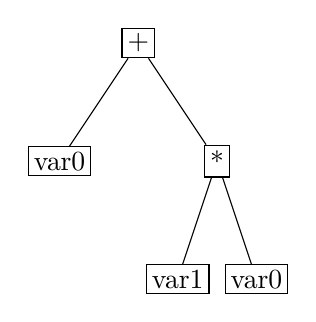
\begin{tikzpicture}
        [
        every node/.style={draw, inner sep=2pt},
        level distance=1.5cm,
        level 1/.style={sibling distance=2cm},
        level 2/.style={sibling distance=1cm}
        ]
        
        \node {+}
        child {
            node {var0}
        }
        child {
            node {*}
            child {
            node {var1}
            }
            child {
            node {var0}
            }
        };
    \end{tikzpicture}
    \caption{An example of an abstract syntax tree (AST). This translates to the function \texttt{f = var0 + var1 * var0}.}
    \label{fig:AST}
\end{figure}








% \begin{figure}[H]
%     \centering
%     \begin{tikzpicture}
%         [
%         every node/.style={draw, inner sep=2pt},
%         level distance=1.5cm,
%         level 1/.style={sibling distance=2cm},
%         level 2/.style={sibling distance=1cm}
%         ]
        
%         \node {map}
%         child {
%             node {var0}
%         }
%         child {
%             node {*}
%             child {
%             node {var1}
%             }
%             child {
%             node {var0}
%             }
%         };
%     \end{tikzpicture}
%     \caption{An example of an abstract syntax tree (AST). This translates to the function \texttt{f = var0 + var1 * var0}.}
%     \label{fig:AST}
% \end{figure}





% All modules are written using PyTorch \cite{NEURIPS2019_9015}.





\paragraph*{Generative Model}\label{sec:gen_model}
To embed programs effectively within a neural network, it is essential to represent them in a format that is compatible with the neural network's architecture. Abstract syntax trees, which are inherently 2-dimensional and include information of parent, children and sibling nodes, should be translated into a neural network format while ensuring the preservation of this valuable structural information.
Various concepts have emerged, including using \acrfullpl{gnn}, see e.g. \cite{allamanis_learning_2018,velickovicCLRSAlgorithmicReasoning2022,bieber_learning_2020,ibarz_generalist_2022}. Others proposed special Tree-Transformers which are able to encode \acrshortpl{ast}, see e.g. \cite{pengRethinkingPositionalEncoding2022,wang2017dynamic}.
\citet{heTreesTransformersTheoretical2021} find that standard Transformers achieve similar results to Transformers where tree position information is explicitly encoded. This is presumably because of the positional encoding, which is a way of adding fixed sinusoidal functions with different frequencies and phases to the embeddings of tokens in a sequence, enabling the neural network to discern the position of each tokens through these distinctive patterns; and more importantly, because of the fundamental component of the Transformer, which is the self-attention mechanism, formalized as \cite{vaswaniAttentionAllYou2017}:
\begin{equation}
    \text{Attention}(Q, K, V) = \text{softmax}(\frac{QK^T}{\sqrt{d_k}})V
\end{equation}

This mechanism, through the query (Q), key (K), and value (V) matrices, allows the model to dynamically assign importance to different parts of the input sequence. The scaling factor $\sqrt{d_k}$ normalizes the dot product, aiding in stabilizing gradients during training. Moreover, the Transformer employs Multi-Head Attention, enabling the model to concurrently process information from different representation subspaces, enhancing its capability to capture diverse features. 
Therefore, I decided to use the standard Transformer architecture, which takes a 1-dimensional sequence as an input, meaning the \acrshort{ast} has to be linearized. 

Rather than embedding the primitives of the DSL to construct \acrshortpl{ast}, the already preprocessed rules of the context-free grammar are embedded, created in conjunction with the syntactic constraints, thus essentially predicting edges rather than nodes. The array of \acrshort{cfg} rules has to be converted back to \acrshort{ast} format for evaluation, which can be easily done within the DeepSynth framework.
In a plausible model of cognition, we don't possess an explicit representation of the \acrshort{cfg} but rather infer it.
However, in the case of DeepSynth, it generates a more extensive \acrshort{cfg} instead of conducting type inference, which is the approach employed in DreamCoder. Consequently, a lookup to identify the syntactically permitted rules must be performed, thereby filtering out those that do not conform to the syntax. Naturally, in principle the model could be allowed to generate syntactically incorrect programs and assign them a reward of 0 during evaluation, but to expedite the learning process, I refrain from doing so.

\begin{description}
    \item[The RuleEncoder] begins by collecting rules, which are pairs of non-terminals and corresponding program actions, from the \acrshort{cfg} and adds special tokens such as 'PAD' (padding), 'START' (sequence start), and 'STOP' (sequence end). Each rule is passed through an embedding layer.
    During the forward pass, batches of state sequences (each state sequence, or trajectory $\tau$, representing a series of \acrshort{cfg} rules) are processed. To ensure uniformity across different sequences within a batch, padding is applied.
    \item[The IOEncoder] is tasked with encoding \acrfull{io} pairs into continuous vector representations.
    Each input-output pair is tokenized using a predefined lexicon (a list of symbols representing the possible range of inputs and outputs), which includes special tokens such as 'PAD' (padding), 'IN' (input start), and 'OUT' (output start). This tokenization is critical for distinguishing between different parts of the input-output pairs.
    The tokenized input-output pairs are concatenated into a single sequence, with the 'IN' and 'OUT' tokens demarcating the transition from input to output. Padding is then applied to ensure that all sequences have the same length, aligning them to the maximum allowed size determined by \texttt{n\_examples\_max} (the maximum number of input examples that can be processed) and \texttt{size\_max} (the maximum size of elements in a list). These parameters have been adapted from DeepSynth. The padded sequences are passed through an embedding layer. This embedding is crucial for capturing the semantic relationships between different tokens.
    \item[The Transformer] initializes with the IOEncoder and the RuleEncoder. Positional Encoding is applied to the output of both encoders. This step is vital as it adds information about the sequence order to the model, allowing the Transformer to interpret the sequence data effectively.
    The Transformer employs two types of masks: padding masks for IO sequences and square subsequent masks for state sequences. The padding mask ensures that the model does not process padding tokens, while the square subsequent mask prevents positions from attending to subsequent positions, maintaining the autoregressive property in the generation process.
\end{description}

\paragraph*{Forward Policy}
At each step, the forward policy takes the Transformer output as an encoded state and predicts log probabilities over the \acrshort{cfg} rules, after which softmax is applied to get a distribution between 0 and 1 and sample the next action. 
The forward policy is implemented as a \acrfull{mlp} and predicts forward logits from the Transformer's output, guiding the generative process.

\paragraph*{Partition Function}
The partition function $Z_\theta$, which is an estimation of the sum of all rewards $R(\rho|x)$, serves as a normalizing factor, ensuring that the probabilities generated by the model are well-calibrated and interpretable. It is implemented as a \acrshort{mlp} layered on top of the Transformer, outputting a scalar.

See \autoref{table:params} for the exact parameterization of the models.

\paragraph*{Sampling Programs}\label{sec:sampling_programs}
In the process of constructing an Abstract Syntax Tree, there exists flexibility in the order of expansion. Nodes can be expanded in a depth-first, breadth-first, etc. manner, or for instance, one can adopt a bottom-up approach, wherein terminal nodes are predicted initially and subsequently connected in a progressive manner. This approach offers the advantage of enabling the evaluation of partial expressions, which, in turn, can serve to inform the model and enhance computational efficiency, albeit at the expense of increased memory requirements. Alternatively, we may consider employing a model akin to the forward policy, predicting the subsequent node (or edge) to be expanded.
However, I chose to sample the actions for the tree construction in a depth-first manner, mainly for two reasons. 
First, for simplicity, and second so that the AST when linearized always has the same order, potentially giving the Transformer a useful inductive bias.

Specifically, the state of each program in the batch is initialized with a 'START' token, representing the initial state of the program generation process. A frontier, implemented as a queue, is initialized for each program to manage the sequence of non-terminals that need to be expanded. This method has been adapted from DeepSynth to fit with the FlowCoder framework and mechanisms. 
The core of the method is a loop that continues until all frontiers are empty, indicating that all programs in the batch have been fully generated. Within this loop, the model computes logits and partition functions.
The sampling method includes an exploration mechanism, where with a probability $\epsilon$, uniform sampling is used instead of the model's logits. This exploration is crucial for introducing variability and avoiding local optima in the generation process. Additionally, tempering is applied to logits using a factor $\beta$, modulating the sharpness of the probability distribution used for sampling.
For each program in the batch, the method iteratively samples a rule based on the current non-terminal and updates the program's state and cumulative logits. This process involves creating a mask to block invalid actions, applying the mask to logits, and sampling an action (rule) based on the masked logits.
Each sampled rule is decomposed into a non-terminal and program component, updating the program's current state and expanding the frontier with the rule's arguments.
Once all frontiers are empty, the final programs are reconstructed from their compressed representations, using methods provided by DeepSynth.

\paragraph*{Reward} \label{sec:reward}
In order to train the model, a reward function has to be operationalized. Various approaches exist for this purpose, the simplest being a binary reward, as employed in DreamCoder. Does the output of the program match the actual output or not? A binary reward however, is not very informative. A reward that provides a gradient is much more useful. \citet{bengioGFlowNetFoundations2023} propose an \acrfull{ebm}, wherein the model learns to associate favorable outcomes with low energy states and unfavorable outcomes with high energy states. I found that this method introduced unnecessary complexity to the model. Instead, the Levenshtein edit distance was used \footnote{The implementation of the Levenshtein distance I used can be found at \url{https://github.com/maxbachmann/Levenshtein}}, which is a measure of the similarity between two strings \cite{Levenshtein}. Specifically, it quantifies the minimum number of single-character edits (i.e., insertions, deletions, or substitutions) required to transform one string into another. See the appendix (\autoref{app:levenshtein}) for an in depth formalization of the metric.
Since the Levenshtein distance returns a discrete value, it was normalized over the maximum length of the sequences, and since there may be more than one example per task, it was averaged over all examples. Moreover, a maximum reward parameter was applied, to scale a correct solution up and give the model a stronger gradient. In my experiments a maximum reward of 10 was used.


\subsection{Design} \label{subsec:design}
In the following section I will elaborate on the exact training and test methods employed, including hyperparameters.
The tasks that were used are input-output relations in the list editing domain, originally from DreamCoder, see \autoref{tab:task_ex} for examples. These were filtered given the syntactic constraints (e.g. type, lexicon, etc.) and provided by DeepSynth. 
In their paper, \citet{fijalkowScalingNeuralProgram2021} discuss that some of the tasks are impossible to solve given the DSL, therefore, those were additionally filtered out, finally leaving 95 tasks in the dataset. Tasks can be of a similar variety (e.g. \texttt{add-k with k=1} and \texttt{add-k with k=2} belong to the same group). There are 25 such task groups in total. Each task can have between 1 and 15 examples. A task is considered solved if a program solves all examples of the task \footnote{All tasks can be found in my GitHub repository.}.
The DSL is essentially a dictionary of primitive types and semantics in a typed $\lambda$-calculus, including functions like \texttt{index}, \texttt{car}, \texttt{append} as well as numerical functions like \texttt{+}, \texttt{*}, \texttt{mod}, \texttt{is-prime}, etc., all written in Python (\autoref{app:dsl}).
\autoref{tab:synconst} describes the syntactical constraints used in the experiment, which were mostly adapted from DeepSynth and DreamCoder.

\begin{table}[H]
    \centering
    \begin{tabularx}{\textwidth}{|l|l|X|}
        \hline
        \textbf{Parameter} & \textbf{Value} & \textbf{Description} \\\hline
        \texttt{type} & \texttt{list(int) $\rightarrow$ list(int)} & The input as well as the output should be a list of integers, so the CFG should reflect that, filtering rules that do not conform to that criterion. \\\hline
        \texttt{lexicon} &  $[-30, 30] \in \mathbb{Z}$ & The lexicon is a uniform distribution of integers and in the range from -30 to 30 \\\hline
        \texttt{maximum argument number} & 1 & This is the maximum number of arguments a function could have. \\\hline
        \texttt{size max} & 10 & The maximum number of values in a list \\\hline 
        \texttt{max number of examples} & 15 & The maximum number of examples per task \\\hline 
    \end{tabularx}
    \caption{Syntactical Constraints}
    \label{tab:synconst}
\end{table}

All experiments were trained in random order with a batch size of 4 where each task in the batch is the same. This was done to avoid a credit assignment problem while increasing efficiency. Since the forward logits are summed up and averaged over for all trajectories, training the model at multiple task at once might have confused which trajectory was rewarding. However, batching, especially when training on a GPU has computational benefits.
Furthermore, each task is trained for 5 epochs with 2.000 E-steps and 2.000 M-steps in each epoch. The moving average threshold (see \autoref{eq:threshold}) $\delta$ was initialized with 150 and linearly decreases using the hyperparameter $\alpha$ set to $0.3$. The exploration parameters $\beta$ and $\epsilon$ were set to $0.7$ and $0.3$, respectively. The sleep weight $\gamma$ was set to 10 on all experiments. 
The learning rates for the generative model as well as for the forward policy were set to $0.0001$. During inference I ran the model for $100$ steps. Since the batch size is 4, this creates 400 programs per task. A table of all hyperparameters can be found in \autoref{app:hyperparams}. The experiments were run on a single NVIDIA Tesla T4 GPU. Throughout the five epochs, each consisting of 2.000 E- and M-steps with a batch size of four, the model generated approximately 80.000 programs per task.

\begin{table}[ht]
    \centering
    \begin{tabular}{|p{5cm}|c|c|}
        \hline
        \textbf{Task} & \textbf{Input} & \textbf{Output} \\\hline
        \texttt{remove gt 2} & \texttt{[1,2,7,5,1]} & \texttt{[1,2,1]} \\\hline
        \texttt{caesar-cipher-k-modulo-n with k=5 and n=4} & \texttt{[2, 2, 0, 1, 2, 3, 3]} & \texttt{[3, 3, 1, 2, 3, 0, 0]} \\\hline
        \texttt{prepend-index-k with k=3} & \texttt{[15, 12, 9, 14, 7, 9]} & \texttt{[9, 15, 12, 9, 14, 7, 9]} \\\hline
        \texttt{add-k with k=4} & \texttt{[16, 10, 7, 12, 13, 3]} & \texttt{[20, 14, 11, 16, 17, 7]} \\\hline
        \texttt{append-k with k=2} & \texttt{[1, 5, 15]} & \texttt{[1, 5, 15, 2]} \\\hline
    \end{tabular}
    \caption{Task Examples}
    \label{tab:task_ex}
\end{table}


\begin{table}[ht]
    \centering
    \begin{tabular}{|p{5cm}|c|}
        \hline
        \textbf{Task} & \textbf{Program} \\\hline
        \texttt{remove gt 2} & \texttt{(filter (gt? 3) var0)} \\\hline
        \texttt{caesar-cipher-k-modulo-n with k=5 and n=4} & \texttt{(map (mod 4) (map (+ 5) var0))} \\\hline
        \texttt{prepend-index-k with k=3} & \texttt{(cons (index 2 var0) var0)} \\\hline
        \texttt{add-k with k=4} & \texttt{(map (+ 4) var0)} \\\hline
        \texttt{append-k with k=2} & \texttt{(append 2 var0)} \\\hline
    \end{tabular}
    \caption{Examples of tasks and programs solving the tasks.}
    \label{tab:task_programs}
\end{table}


























% The full algorithm is described in the pseudocode: \autoref{alg:flowcoder}. 



% \begin{algorithm}[H]
%     \caption{FlowCoder}
%     \begin{algorithmic}[1]
%     \Require Data $X$, generative model with parameters $\theta$, forward policy with parameters $\phi$, optimization and exploration hyperparameters, threshold $\alpha$
%     \Repeat
%         \State Sample $x \sim X$
%         \State Sample $z \sim \pi_\phi(z|x)$
%         \State \textbf{E-step}: gradient update on $\phi$ with $\nabla_\phi \mathcal{L}_{TB}$
%         \If{$r \in (0, 1) < \texttt{replay\_prob}$}
%             \State gradient update on $\phi$ with $\nabla_\phi\mathcal{L}_{\text{Replay}}$
%         \EndIf
%         \If{$r \in (0, 1) < \texttt{fantasy\_prob}$}
%             \State gradient update on $\phi$ with $\nabla_\phi\mathcal{L}_{\text{Fantasy}}$
%         \EndIf
%         \If{$\mathcal{L} < \alpha$}
%             \State Sample $z \sim \pi_\phi(z|x)$
%             \State \textbf{M-step}: gradient update on $\theta$ with $\nabla_\theta[-\log p_\theta(x|z)p_\theta(z)]$
%         \EndIf
%     \Until{some convergence condition}
%     \end{algorithmic}
%     \label{alg:flowcoder}
%     \end{algorithm}
% \todo[inline]{explain algorithm, check for additional hyperparameters, etc. should the gradient update of mstep be just the reward? }
























% \begin{figure}
%     \centering
%     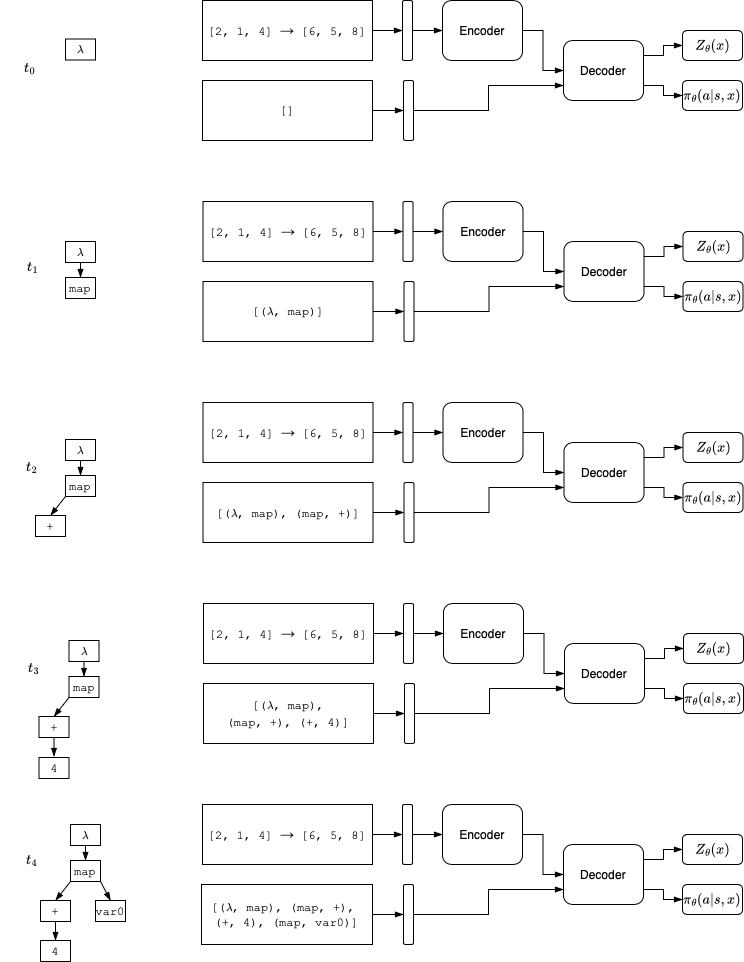
\includegraphics[width=\textwidth]{../img/gflownet.drawio.png}
%     \caption{FlowCoder constructs a program by sequentially encoding a shared task-state representation, from which the forward policy $\pi$ predicts the next action $a$. The complete trajectory}
%     \label{fig:flowchart}
% \end{figure}

























% \begin{figure*}[htbp]
%     \centering
%     \begin{adjustbox}{width=\textwidth}
%         \begin{tikzpicture}[
%             node distance=2cm, 
%             auto, 
%             thick,
%             box/.style={
%                 rectangle,
%                 rounded corners,
%                 draw=black, 
%                 align=center,
%                 drop shadow,
%                 minimum height=1cm,
%                 minimum width=2cm
%             },
%             arrow/.style={
%                 ->,
%                 -{Stealth[length=10pt]}
%             }
%         ]
        
%             % Nodes
%             \node[box, fill=yellow!50] (task) {Task};
%             \node[box, fill=yellow!70, right=3cm of task] (ioencoder) {IOEncoder};
%             \node[box, fill=blue!20, below=1cm of task] (state) {State};
%             \node[box, fill=blue!50, right=3cm of state] (ruleencoder) {RuleEncoder};
            
%             % Positioning the Transformer node in between IOEncoder and RuleEncoder
%             \coordinate (middle) at ($(ioencoder.east)!0.5!(ruleencoder.east)$);
%             \node[box, fill=green!20, right=3cm of middle] (transformer) {Transformer};
            
%             % Nodes for FORWARD and Z at 45 degree angles
%             \node[box, fill=purple!30, above right=0.5cm and 2cm of transformer] (forward) {FORWARD};
%             \node[box, fill=purple!50, below right=0.5cm and 2cm of transformer] (z) {Z};
        
%             % Edges
%             \draw[arrow] (task) -- (ioencoder);
%             \draw[arrow] (state) -- (ruleencoder);
%             \draw[arrow] (ioencoder) -- (transformer);
%             \draw[arrow] (ruleencoder) -- (transformer);
%             \draw[arrow] (transformer) -- (forward);
%             \draw[arrow] (transformer) -- (z);
        
%         \end{tikzpicture}
%     \end{adjustbox}
%     \caption{Insert explanation + maybe change task to an actual task; same with state; maybe also show the forward and Z output better.}
%     \label{ref:model_diagram}
% \end{figure*}
% % \todo[inline]{this looks like its one model show that the transformer output is a state representation. the GFlowNet 
% %  and Z takes it and produces logits.}






% \begin{figure}[H]
%     \centering
%     % Tree 1
%     \begin{subfigure}[t]{0.18\textwidth}
%         \centering
%         \raisebox{1.5cm}{ % Adjust vertical position
%         \begin{tikzpicture}[every node/.style={draw, circle, inner sep=2pt}]
%             \node {+};
%         \end{tikzpicture}
%         }
%         \caption{Step 1}
%     \end{subfigure}
%     \hspace{0.5cm} % Space between trees
%     % Tree 2
%     \begin{subfigure}[t]{0.18\textwidth}
%         \centering
%         \raisebox{0.75cm}{ % Adjust vertical position
%         \begin{tikzpicture}[every node/.style={draw, circle, inner sep=2pt}]
%             \node {+}
%             child { node {var0} };
%         \end{tikzpicture}
%         }
%         \caption{Step 2}
%     \end{subfigure}
%     \hspace{0.5cm} % Space between trees
%     % Tree 3
%     \begin{subfigure}[t]{0.18\textwidth}
%         \centering
%         \begin{tikzpicture}[every node/.style={draw, circle, inner sep=2pt}]
%             \node {+}
%             child { node {var0} }
%             child { node {*} };
%         \end{tikzpicture}
%         \caption{Step 3}
%     \end{subfigure}
%     \hspace{0.5cm} % Space between trees
%     % Tree 4
%     \begin{subfigure}[t]{0.18\textwidth}
%         \centering
%         \raisebox{-0.75cm}{ % Adjust vertical position
%         \begin{tikzpicture}[every node/.style={draw, circle, inner sep=2pt}]
%             \node {+}
%             child { node {var0} }
%             child { node {*}
%                 child { node {var1} }
%             };
%         \end{tikzpicture}
%         }
%         \caption{Step 4}
%     \end{subfigure}
%     \hspace{0.5cm} % Space between trees
%     % Tree 5
%     \begin{subfigure}[t]{0.18\textwidth}
%         \centering
%         \raisebox{-1.5cm}{ % Adjust vertical position
%         \begin{tikzpicture}[every node/.style={draw, circle, inner sep=2pt}]
%             \node {+}
%             child { node {var0} }
%             child { node {*}
%                 child { node {var1} }
%                 child { node {var0} }
%             };
%         \end{tikzpicture}
%         }
%         \caption{Step 5}
%     \end{subfigure}
%     \caption{Incremental construction of the abstract syntax tree (AST) for \texttt{var0 + var1 * var0}.}
%     \label{fig:AST}
% \end{figure}



% \begin{figure}
%     \centering
    
%     % Define styles for the nodes and the level distances
%     \tikzset{
%         every node/.style={draw, circle, inner sep=2pt},
%         level distance=12mm,
%         level 1/.style={sibling distance=24mm},
%         level 2/.style={sibling distance=12mm},
%     }
    
%     % Tree at time t = 1
%     \begin{subfigure}[b]{0.2\textwidth}
%         \centering
%         \begin{tikzpicture}
%             \node {+}
%                 child {edge from parent[draw=none]}
%                 child {edge from parent[draw=none]};
%         \end{tikzpicture}
%         \caption*{$t = 1$}
%     \end{subfigure}
%     \hspace{1em} % Space between trees
%     % Tree at time t = 2
%     \begin{subfigure}[b]{0.2\textwidth}
%         \centering
%         \begin{tikzpicture}
%             \node {+}
%                 child {node {pow}}
%                 child {edge from parent[draw=none]};
%         \end{tikzpicture}
%         \caption*{$t = 2$}
%     \end{subfigure}
%     \hspace{1em} % Space between trees
%     % Tree at time t = 3
%     \begin{subfigure}[b]{0.2\textwidth}
%         \centering
%         \begin{tikzpicture}
%             \node {+}
%                 child {node {pow}}
%                 child {node {y}};
%         \end{tikzpicture}
%         \caption*{$t = 3$}
%     \end{subfigure}
%     \hspace{1em} % Space between trees
%     % Tree at time t = 4
%     \begin{subfigure}[b]{0.2\textwidth}
%         \centering
%         \begin{tikzpicture}
%             \node {+}
%                 child {node {pow}
%                     child {node {y}}
%                     child {edge from parent[draw=none]}
%                 }
%                 child {edge from parent[draw=none]};
%         \end{tikzpicture}
%         \caption*{$t = 4$}
%     \end{subfigure}
    
%     % Tree at time t = 5
%     \begin{subfigure}[b]{0.2\textwidth}
%         \centering
%         \begin{tikzpicture}
%             \node {+}
%                 child {node {pow}
%                     child {node {y}}
%                     child {node {x}}
%                 }
%                 child {edge from parent[draw=none]};
%         \end{tikzpicture}
%         \caption*{$t = 5$}
%     \end{subfigure}
    
%     \caption{Creation of a five node tree using the grow initialization method with a maximum depth of 2, using terminal set $T$ and function set $F$ defined earlier, ($t = $ time).}
%     \label{fig:growth_trees}
%     \end{figure}
    



























% \begin{tikzpicture}[node distance=2cm]

%     % Define styles for boxes, decisions, and lines
%     \tikzstyle{box} = [rectangle, draw=black, thick, minimum height=2em, minimum width=4em, text centered, draw=black]
%     \tikzstyle{line} = [draw, -latex', thick]
    
%     % Define nodes
%     \node (st) {$s_t = $};
%     \node [circle, draw=black, thick, above right of=st, node distance=1cm] (1) {map};
%     \node [circle, draw=black, thick, above right of=1, node distance=1cm] (2) {2};
%     \node [circle, draw=black, thick, below right of=1, node distance=1cm] (3) {3};
%     \node [box, right of=2, node distance=3cm] (gflownet) {GFlowNet $P_F$};
%     \node [right of=gflownet, node distance=3cm] (pi) {$\pi(A|s_t)$};
%     \node [right of=pi, node distance=3cm] (at) {draw $a_t \sim \pi(A|s_t)$};
%     \node [below of=at, node distance=1cm] (at_text) {$a_t =$ ``Add a new node connected to node 2''};
%     \node [below of=st, node distance=4cm] (st1) {$s_{t+1} = $};
%     \node [circle, draw=black, thick, right of=st1, node distance=1cm] (1') {1};
%     \node [circle, draw=black, thick, above right of=1', node distance=1cm] (2') {2};
%     \node [circle, draw=black, thick, below right of=1', node distance=1cm] (3') {3};
%     \node [circle, draw=black, thick, fill=blue, right of=2', node distance=1.5cm] (4) {4};
%     \node [box, right of=4, node distance=3cm] (gflownet2) {GFlowNet $P_F$};
%     \node [right of=gflownet2, node distance=3cm] (pi2) {$\pi(A|s_{t+1})$};
%     \node [right of=pi2, node distance=3cm] (at1) {draw $a_{t+1} \sim \pi(A|s_{t+1})$};
%     \node [below of=at1, node distance=1cm] (at1_text) {$a_{t+1} = \ldots$};
    
%     % Draw edges between nodes
%     \draw [line] (1) -- (2);
%     \draw [line] (1) -- (3);
%     \draw [line] (1') -- (2');
%     \draw [line] (1') -- (3');
%     \draw [line] (2') -- (4);
%     \draw [line] (st) -- (gflownet);
%     \draw [line] (gflownet) -- (pi);
%     \draw [line] (pi) -- (at);
%     \draw [line] (st1) -- (gflownet2);
%     \draw [line] (gflownet2) -- (pi2);
%     \draw [line] (pi2) -- (at1);
    
%     % Draw the arrows for the state transitions
%     \draw [->,thick] (at_text) -- ++(0,-1) -| (st1) node [near start, below] {$T(s_t,a_t)$ determines $s_{t+1}$};
    
% \end{tikzpicture}













% \begin{figure*}[htbp]
%     \centering
%     \begin{adjustbox}{width=\textwidth}
%         \begin{tikzpicture}[level distance=1.5cm,
%             level 1/.style={sibling distance=6cm},
%             level 2/.style={sibling distance=3cm},
%             every node/.style={circle, draw}]
        
%         \node at (-9,0) {$\lambda$};

%         \node at (-6,0) {$\lambda$}
%             child {node {+}};
%         \node at (-3,0) {$\lambda$}
%             child {node {+}
%                 child {node {x}}
%             };
%         \node at (0,0) {$\lambda$}
%             child {node {+}
%                 child {node {x}}
%                 child {node {x}}
%             };
%         \node at (3,0) {$\lambda$}
%             child {node {+}
%                 child {node {x}}
%                 child {node {max}
%                     child {node {x}}
%                     child {node {x}}
%                 }
%             };
%         \node at (6,0) {$\lambda$}
%             child {node {+}
%                 child {node {x}}
%                 child {node {max}
%                     child {node {x}}
%                     child {node {y}}
%                 }
%             };
%         \node at (9,0) {$\lambda$}
%             child {node {+}
%                 child {node {x}}
%                 child {node {max}
%                     child {node {y}}
%                     child {node {x}}
%                 }
%             };
        
%         % Second tree sequence (Figure 6)
%         \node at (-3,-5) {+};
%         \node at (0,-5) {+}
%             child {node {pow}};
%         \node at (3,-5) {+}
%             child {node {pow}
%                 child {node {y}}
%             };
%         \node at (6,-5) {+}
%             child {node {pow}
%                 child {node {y}}
%                 child {node {x}}
%             };
%         \node at (9,-5) {+}
%             child {node {pow}
%                 child {node {y}}
%                 child {node {x}}
%             }
%             child {node {3}};
        
%         \end{tikzpicture}
%     \end{adjustbox}
%     \caption{Creation of trees showing the construction process.}
% \end{figure*}




% \begin{figure}
%     \centering
%     \begin{tikzpicture}[
%       node distance = 2cm,
%       auto,
%       block/.style = {circle, draw, font=\sffamily\Large\bfseries},
%       line/.style = {draw, -latex}
%     ]
    
%     % Nodes
%     \node [block] (S) {S};
%     \node [block, below left of=S] (R1) {R};
%     \node [block, below right of=S] (T1) {T};
%     \node [block, below left of=R1] (R2) {R};
%     \node [block, below right of=R1] (T2) {T};
%     \node [block, below right of=R2] (a) {a};
%     \node [block, right of=a] (b) {b};
    
%     % Paths
%     \path [line] (S) -- node {f(R,T)} (R1);
%     \path [line] (S) -- node {g(T)} (T1);
%     \path [line] (R1) -- node {f(R,T)} (R2);
%     \path [line] (R1) -- node {g(T)} (T2);
%     \path [line] (T2) -- node {a} (a);
%     \path [line] (T2) -- node {b} (b);
    
%     % DFS, BFS, A* paths (without specific details)
%     \draw [red, thick, dashed] (S) to [bend left] (R2);
%     \draw [blue, thick, dashed] (S) to [bend right] (b);
%     \draw [green, thick, dashed] (S) to [bend right] (T2);
    
%     \end{tikzpicture}
%     \caption{Illustration of the tree of leftmost derivations.}
%     \end{figure}































